\section{物理节点单故障可生存性虚拟网络嵌入问题}
\subsection{问题描述}

\begin{frame}{目录}
    \setbeamertemplate{section in toc}[sections numbered]
    \tableofcontents[currentsection,hideothersubsections]
\end{frame}
\addtocounter{framenumber}{-1}  %目录页不计算页码

\begin{frame}
\frametitle{虚拟网络请求}
\textbf{虚拟网络}VN表示为无向图$G (V,E)$,其中$V$ 和$E$ 分别是虚拟节点和虚拟链路的集合。每个虚拟链路$e_{ij}$具有带宽需求$d_{ij}$。 每个虚拟节点$v_i$ 具有计算容量需求$d_i$。 对于虚拟节点$v_i$,需要在虚拟节点上执行的虚拟功能表示为$f(i)$。
\begin{figure}[htbp]
\centering
% Requires \usepackage{graphicx}
\includegraphics[width=1.9in]{figures/VirtualNetworkRequest}\\
\caption{虚拟网络请求$G(V,E)$
}\label{fig:VirtualNetworkRequest}
\end{figure}
\end{frame}

\begin{frame}
\frametitle{底层物理网络}
\textbf{物理网络}建模为一个无向图$G (S,L)$,其中$S$ 和$L$ 分别是物理节点和物理链路的集合。对于物理节点$s_i$,我们使用$F(i)$ 和$c_i$分别表示可以在该节点上执行的一组可行的虚拟功能和可用的计算能力。每个物理链路$l_{ij}$ 都有可用带宽$b_{ij}$。
\begin{figure}[htbp]
\centering
% Requires \usepackage{graphicx}
\includegraphics[width=3.0in]{figures/PhysicalNetwork}\\
\caption{底层物理网络$G(S,L)$}\label{fig:PhysicalNetwork}
\end{figure}
\end{frame}


\begin{frame}
\frametitle{虚拟网络嵌入}
给定VN请求$G (V,E)$情况下,虚拟网络嵌入问题的目的是将该请求映射到物理网络$G (S,L)$ 上,同时提供所需的足够资源。可行的嵌入应该满足节点容量约束、链路带宽约束和功能类型约束这三个约束条件。
\begin{figure}[htbp]
\centering
% Requires \usepackage{graphicx}
\includegraphics[width=2in]{figures/VirtualNetworkEmbedding}\\
\caption{虚拟网络嵌入}\label{fig:VirtualNetworkEmbedding}
\end{figure}
\end{frame}

%\begin{frame}
%  对于VN请求$G (V,E)$和物理网络$G (S,L)$,给出了其占用物理网络的可行映射,在任何一个物理节点发生故障时,增加最小备份物理资源以提供可生存性的网络服务。
%
%  NP-hard?? ILP很难解
%\end{frame}

\subsection{原有算法}
\begin{frame}
\frametitle{原有算法}
\begin{enumerate}
  \item $\SecondAlgorithmMethodAbrreviation$ :算法将备份节点与关键节点之间、备份节点与备份节点之间的连接起来,而不连接关键节点与关键节点之间,关键节点表示嵌入物理节点中的虚拟节点,备份节点表示增广节点。
  \item $\FouthAlgorithmMethodAbrreviation$:1+1-保护机制,当与虚拟节点映射的底层物理上的每个节点失效时,一种简单的方法是增加一个新的物理节点,用于迁移失败的虚拟节点,并将新的链路与失败的物理节点连接起来。
\end{enumerate}
\end{frame}
\begin{frame}

\begin{figure}[htbp]
\centering
\includegraphics[width=3.8in]{figures/One2OneProtection}\\
\caption{1+1-保护机制}\label{fig:One2OneProtection}
\end{figure}
\end{frame}

\subsection{星型图分解动态规划节点嵌入算法}
\subsubsection{基于星型图的分解}
\begin{frame}
\frametitle{设计思想}
\begin{itemize}
  \item 保证局部拓扑结构来保证全部拓扑结构,提出分解原图的方法。
  \item 每个局部结构之间需要协调。
  \item 通过动态规划来实现节点的映射问题。
\end{itemize}

\end{frame}

%\begin{frame}
%\frametitle{星型图定义}
%\begin{equation}
%VirtualStar(v_i)=(v_i, \phi(v_i), d_i, f_i, D_i, N_i)
%\label{eq:virtualstar}
%\end{equation}
%\begin{equation}
%PhysicalStar(s_j)=(s_j, \phi^{-1}( s_j), c_j, F(j), \phi(N(\phi^{-1}( s_j))), a)
%\label{eq:physicalstar}
%\end{equation}
%\end{frame}

\subsubsection{构建星型二分图}
\begin{frame}
\frametitle{构建星型二分图}
  \begin{figure}
\centering
% Requires \usepackage{graphicx}
\includegraphics[width=3.0in]{figures/StarRepresentation}\\
  \caption{当物理节点$s_1$ 失效时VirtualStar($v_i$)和PhysicalStar($s_j$)}\label{fig:StarRepresentation}
\end{figure}
\begin{equation}
VirtualStar(v_i)=(v_i, \phi(v_i), d_i, f_i, D_i, N_i)
\label{eq:virtualstar}
\end{equation}
\begin{equation}
PhysicalStar(s_j)=(s_j, \phi^{-1}( s_j), c_j, F(j), \phi(N(\phi^{-1}( s_j))), a)
\label{eq:physicalstar}
\end{equation}
\end{frame}

%\begin{frame}
%\frametitle{二分图权值设置}
%公式\ref{eq:edge weight}所示在两种不同的情况下定义了边权重$w(i,j)$。
%\begin{equation}
%w(i,j) = \left\{ {\begin{array}{*{20}{c}}
%   { \alpha \sum\limits_{\phi ({v_k}) \notin \phi (N({\phi ^{ - 1}}({s_j})))} {{d_{ik}}} } & {{v_i} \in {\phi ^{ - 1}}({s_j}),v_k \in N(i)}  \\
%   {\alpha \sum\limits_{k \in N(i)} {{d_{ik}}}  + \beta {M_m} + \lambda {c_i} + \theta } & {{v_i} \notin {\phi ^{ - 1}}({s_j}),v_k \in N(i)}  \\
%\end{array}} \right.
%\label{eq:edge weight}
%\end{equation}
%在公式.(\ref{eq:edge weight})中,$\theta$ 被定义如下.
%\begin{equation}
%\theta  = \left\{ {\begin{array}{*{20}{c}}
%   {{C_s}} & {a = 0}  \\
%   0 & {a = 1}  \\
%\end{array}} \right.
%\end{equation}
%\end{frame}

\begin{frame}
\frametitle{多背包问题定义}
\begin{equation}
\huge{
\begin{array}{*{20}{c}}
   {\mathop {\min }\limits_{{M_{ij}}} } & {\sum\limits_{i = 1}^n {\sum\limits_{j = 1}^m {{M_{ij}}{w_{ij}}} } }  \\
   {s.t.,} & {\sum\limits_{i = 1}^n {{d_i}{M_{ij}}}  \le {c_j}}  \\
   {} & {\sum\limits_{j = 1}^m {{M_{ij}}}  \le 1}  \\
   {} & {{M_{ij}} = \{ 0,1\} }  \\
\end{array}
}
\label{eq:problem formulation}
\end{equation}
\end{frame}

\subsubsection{动态规划节点嵌入}

%\begin{frame}
%
%在等式\ref{eq:place i to j}中,如果物理节点$x_j$的容量限制大于容量需求$d_i$ 并且在物理节点${f_i} \in {F_j}$能执行虚拟功能$f_i$,则 $\theta (i,j)$ 是已经放置前面i−-1 个最佳虚拟星型图的代价和(即$dp[i-1][{x_1} - {d_i}][{x_2}] \ldots [{x_m}]$) 和将虚拟星型图($v_i$) 映射到物理星型图($s_1$)的成本(即$w_{i1}$)。基于$\theta (i,j)$,$dp[i][{x_1}][{x_2}] \ldots [{x_m}]$可通过以下动态规划函数计算。
%\begin{equation}
%dp[i][{x_1}][{x_2}] \ldots [{x_m}] = min\{\theta (i,1),\theta (i,2),\ldots,\theta (i,j),\ldots,\theta (i,m)\}
%\label{eq:update function}
%\end{equation}
%\end{frame}
%
%\begin{frame}
%第$i$个虚拟节点可以选择放置在任何一个存活的的物理星型图上。设$\theta (i,j)$ 表示已经将原先$i-1$个虚拟节点最佳放置后再将第$i$ 个虚拟节点放置到第j 个物理节点的备份资源成本。$\theta (i,j)$表示如下:
%\begin{equation}
%\theta (i,j) = \left\{ {\begin{array}{*{20}{c}}
%{dp[i - 1][x_1][{x_2}] \ldots [{x_j} - {d_i}] \ldots [{x_m}] + {w_{ij}}}\\
%\infty
%\end{array}} \right.\begin{array}{*{20}{c}}
%{({x_j} \ge {d_i},{f_i} \in {F_j})}\\
%{otherwise}
%\end{array}
%\label{eq:place i to j}
%\end{equation}
%\end{frame}


\begin{frame}
\frametitle{多背包问题动态规划解法}
\begin{figure}[htbp]
\centering
% Requires \usepackage{graphicx}
\includegraphics[width=4.5in]{figures/DPIllustration}\\
  \caption{动态规划方法的演示}\label{fig:DPIllustration}
\end{figure}
\end{frame}

\begin{frame}
\begin{algorithm}[H]
\label{alg:DPAlg}
\caption{基于动态规划方法二分星型图匹配算法}
\tiny{
\begin{algorithmic}[1]
\REQUIRE {$dp[i][{x_1}][{x_2}] \ldots [{x_m}]=0(1\leq i \leq n, 0\leq x_1\leq c_1, 0\leq x_2\leq c_2,\ldots, 0\leq x_m\leq c_m)$ 首先被定义成无穷大$\infty$,$dp[0][{x_1}][{x_2}] \ldots [{x_m}]=0(0\leq x_1\leq c_1, 0\leq x_2\leq c_2,\ldots, 0\leq x_m\leq c_m)$, m:物理节点的数量。 $M[{x_1}][{x_2}] \ldots [{x_m}]=\textbf{0}_{n\times m}$ 每个节点的映射矩阵}
\ENSURE {当节点容量为$c_1,c_2,\ldots,c_m$时最小代价的节点映射}
\FORALL{$i$ such that $1\leq i\leq n$ }
\FORALL{$x_1,x_2,\ldots,x_m$ such that $ c_1\geq x_1\geq d_i$, $c_2\geq x_2\geq d_i$,$c_3\geq x_3\geq d_i$,$c_m\geq x_m\geq d_i$}
\STATE{$dp[i][{x_1}][{x_2}] \ldots [{x_m}] = min\{\theta (i,1),\theta (i,2),\ldots,\theta (i,j),\ldots,\theta (i,m)\}$}
\STATE{$j' = \mathop {\arg \min }\limits_j \{\theta (i,1),\theta (i,2),\ldots,\theta (i,j),\ldots,\theta (i,m)\}$, }.
\STATE{$M[{x_1}][{x_2}] \ldots [{x_m}]=M[{x_1}][{x_2}] \ldots[x_{j'}-d_i]\ldots [{x_m}]$}
\STATE{$M[{x_1}][{x_2}] \ldots [{x_m}]_{ij'}=1$}
\ENDFOR
\ENDFOR
\RETURN{$dp[i][{c_1}][{c_2}] \ldots [{c_m}]$ and $M[{c_1}][{c_2}] \ldots [{c_m}]$}
\end{algorithmic}
}
\end{algorithm}
\end{frame}

\begin{frame}
\frametitle{可生存性虚拟网络嵌入算法}
\begin{algorithm}[H]
\label{alg:SeVNAlg}
\caption{星型图分解动态规划节点嵌入算法}
\tiny{
\begin{algorithmic}[1]
\REQUIRE $G (V,E)$:虚拟网络请求; $G (S,L)$:物理网络。
\ENSURE 生成SeVN并增加资源将SeVN嵌入到底层物理网络中。
\STATE 将虚拟网络$G^V$ 嵌入到底层网络$G^S$中
\STATE 从与此VN嵌入请求对应的SN中提取嵌入的虚拟网络eVN$G\left( {\hat S,\hat L} \right)$
%\STATE AllMinimumCycle($G(V,E)$)
\FORALL{$v_i$ 并且 $v_i\in G\left( {\hat S,\hat L} \right)$}
\STATE  从图 $G\left( {\hat S,\hat L} \right)$中分解 eVN $G\left( {\hat S,\hat L} \right)$ 成两个星型结构集 $VirtualStar(v_i)$ 和 $PhysicalStar(s_j)$
\STATE 构建items根据星型结构集 $VirtualStar(v_i)$.
\STATE 构建knapsacks根据星型结构集$PhysicalStar(s_j)$
\STATE 构建边权值矩阵
\STATE 动态规划方法解决多背包问题
\STATE 添加新节点,连接新的边,重新分配节点计算资源和链路的带宽资源到$G\left( {\hat S,\hat L} \right)$中构建新的$G\left( {\hat S,\hat L} \right)$
\ENDFOR
\STATE 从 $G\left( {\hat S,\hat L} \right)$中嵌入增广资源到物理网络$G(S,L)$
\end{algorithmic}
}
\end{algorithm}
\end{frame}

\subsection{算法性能评估及比较}
%\begin{frame}
%\frametitle{实验仿真}
%%所有仿真都运行在服务器上,服务器配置为Intel(R) Xeon(R) CPU E5-2620 2.00GHz (24 Cores) 和 32.00GB RAM。
%
%%对于任何VN请求,VN节点的数目是由3到10之间的均匀分布随机得到的,每一对虚拟节点都是以概率0.5 随机连接的。VN节点的计算需求从1到5 之间随机分布,并且VN 上的带宽从1到10之间随机分布。
%
%%VN请求的到达服从泊松过程(平均每1时间单位请求15次)。请求的持续时间服从指数分布,平均100个时间单位,高的请求率和较长的租用时间保证了物理基础设施的高利用率。
%
%%根据\cite{yu2010survivable},即$\lambda/\alpha=\RelativeCostbetweenComputingBandwidth$,节点的计算资源与链路的带宽资源的相对成本为3。 使用的SN 拓扑是SNDlib拓扑数据\cite{orlowski2010sndlib}如表\ref{tab:SNDlibTopo}所示。 底层物理节点(链路)的计算(带宽)资源都是整数的。分别分布在10至20(50 至100)之间。为了对设备节点失效场景进行建模,我们选择了底层物理网络中的所有底层物理设备节点逐个失效,并统计了每$\SubStrateFacilityNodeFailDuration$个时间单元的迁移频率。
%\begin{table}[htb]
%\centering
%\small{
%\caption{SNDlib拓扑数据}\label{tab:SNDlibTopo}
%\begin{tabular}{|c|c|c|}
%  \hline
%  % after \\: \hline or \cline{col1-col2} \cline{col3-col4} ...
%  数据集 & 节点 & 链路 \\
%  \hline
%  cost266& 37& 57\\
%  geant& 22& 36\\
%  germany50& 50& 88\\
%  giul39& 39& 172\\
%  janos-us-ca& 39& 122\\
%  janos-us& 26& 84\\
%  nobel-eu& 28& 41\\
%  norway& 27& 51\\
%  pioro40& 40& 89\\
%  ta1& 24& 55\\
%  ta2& 65& 108\\
%  zib54& 54& 81\\
%  \hline
%
%\end{tabular}
%}
%\end{table}
%\end{frame}



\begin{frame}
\frametitle{接受率}
\begin{figure}[htbp]
\centering
\begin{minipage}{0.4\textwidth}
\centering
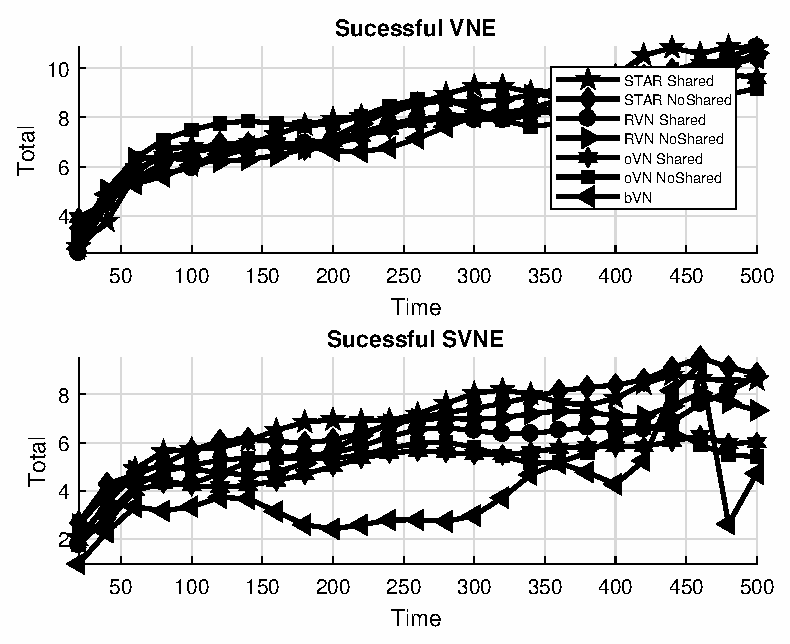
\includegraphics[width=\textwidth]{figures/VirNetReqSurNetReq}
\caption{成功的VNE请求数和成功的SVNE请求数}\label{fig:VirNetReqSurNetReq}
\end{minipage}
\begin{minipage}{0.4\textwidth}
\centering
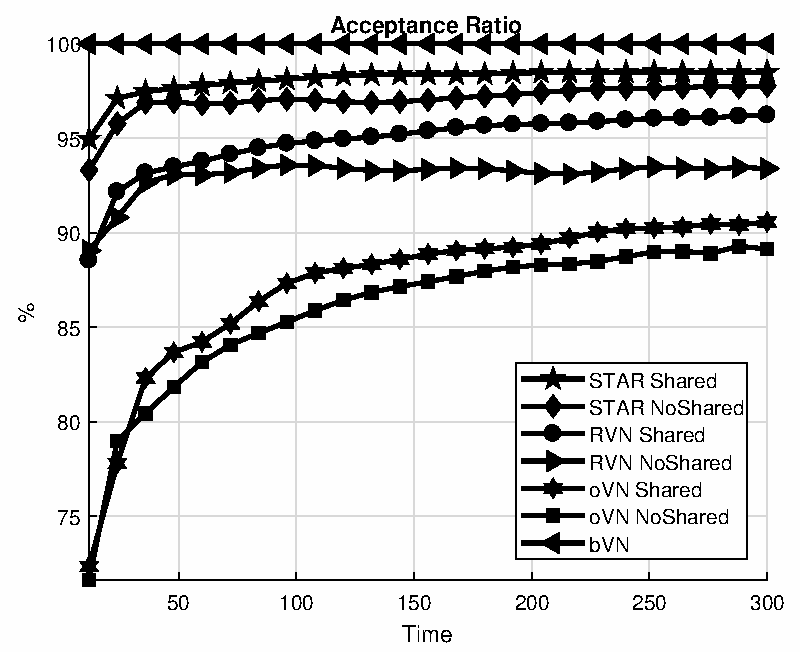
\includegraphics[width=\textwidth]{figures/AcceptionRatio}
\caption{接受率}\label{fig:AcceptionRatio}
\end{minipage}\vspace{\baselineskip}
\end{figure}
\end{frame}


\begin{frame}
\frametitle{活动节点}
\begin{figure}[htbp]
\centering
\begin{minipage}{0.4\textwidth}
\centering
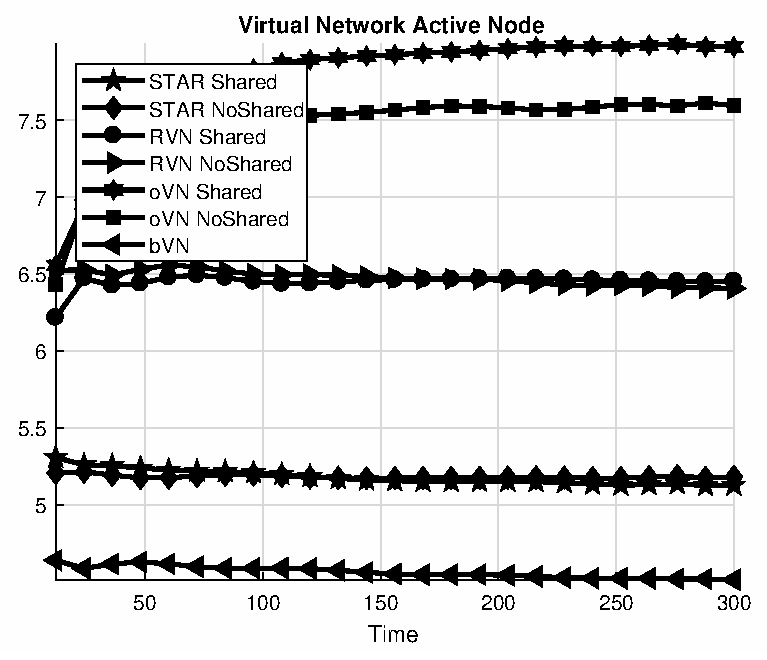
\includegraphics[width=\textwidth]{figures/ActiveNodeAverageVirtualNetwork}
\caption{虚拟网络的平均虚拟节点数}\label{fig:ActiveNodeAverageVirtualNetwork}
\end{minipage}
\begin{minipage}{0.4\textwidth}
\centering
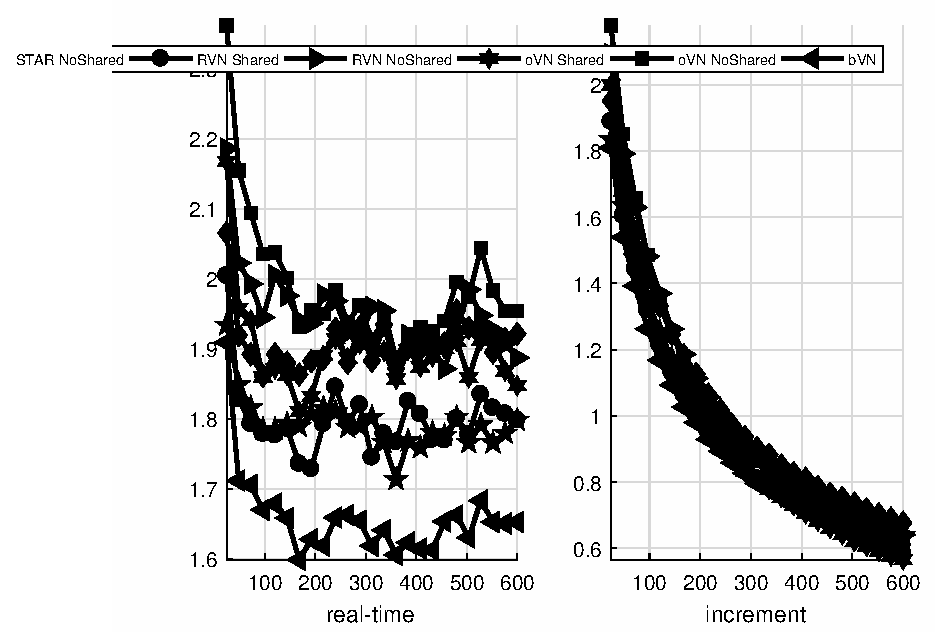
\includegraphics[width=\textwidth]{figures/ActiveNodeAverageSubstrateNetwork}
\caption{底层物理网络平均启动的节点数}\label{fig:ActiveNodeAverageSubstrateNetwork}
\end{minipage}
\begin{minipage}{0.4\textwidth}
\centering
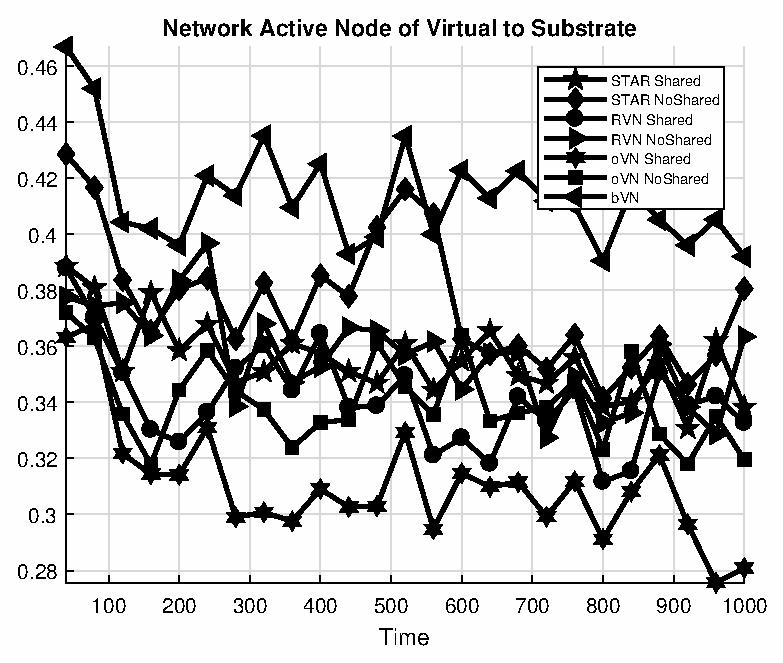
\includegraphics[width=\textwidth]{figures/ActiveNodeSubVir2VirNet}
\caption{底层物理网络启动的节点数与虚拟网络虚拟节点数之比}\label{fig:ActiveNodeSubVir2VirNet}
\end{minipage}\vspace{\baselineskip}
\end{figure}
\end{frame}

\begin{frame}
\frametitle{路径长度}
\begin{figure}[htbp]
\centering
\begin{minipage}{0.4\textwidth}
\centering
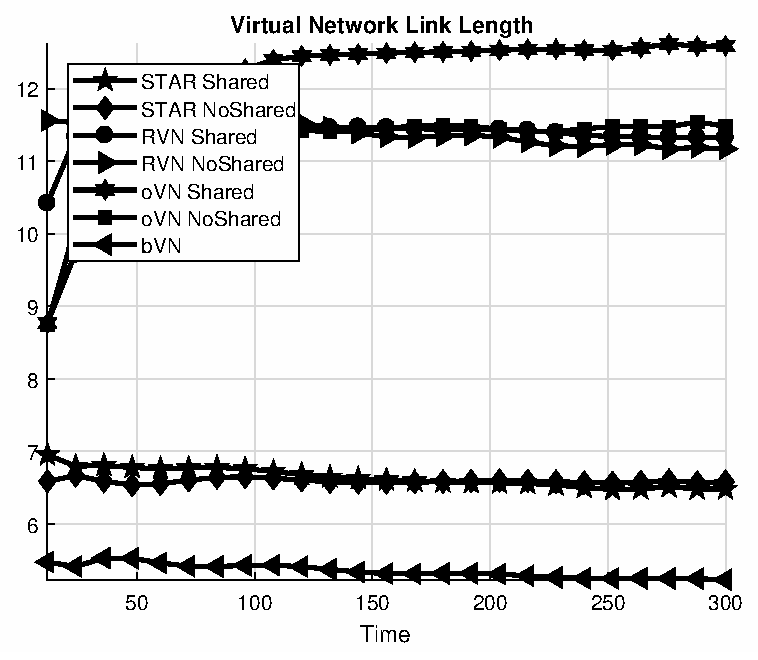
\includegraphics[width=\textwidth]{figures/PathLengthAverageVirtualNetwork}
\caption{虚拟网络链路数}\label{fig:PathLengthAverageVirtualNetwork}
\end{minipage}
\begin{minipage}{0.4\textwidth}
\centering
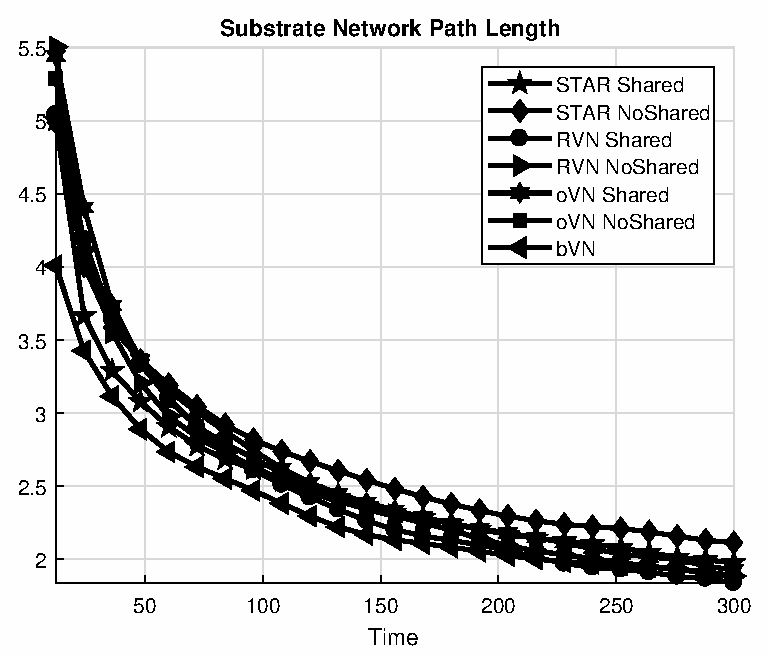
\includegraphics[width=\textwidth]{figures/PathLengthAverageSubstrateNetwork}
\caption{物理网络链路数}\label{fig:PathLengthAverageSubstrateNetwork}
\end{minipage}
\begin{minipage}{0.4\textwidth}
\centering
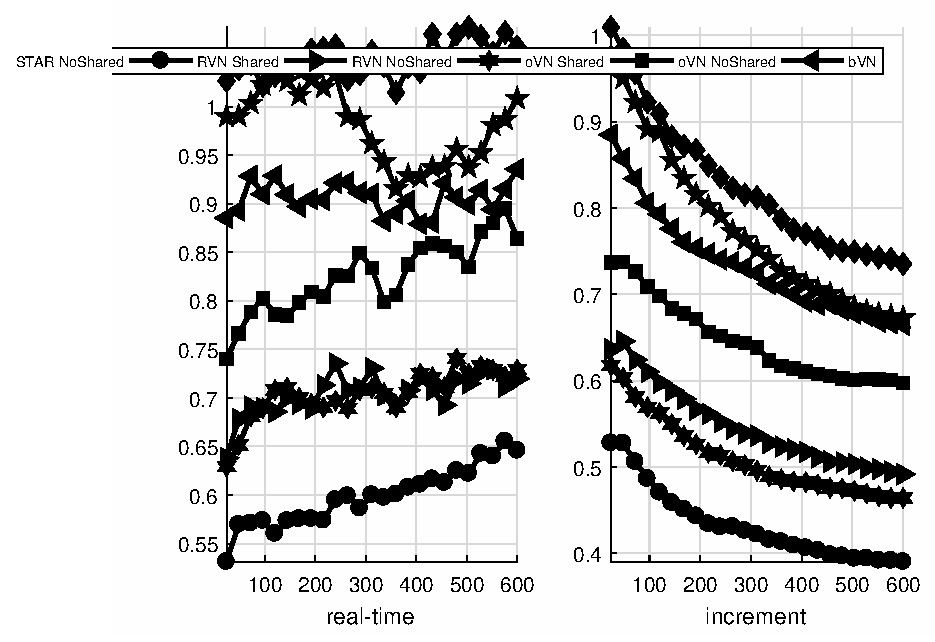
\includegraphics[width=\textwidth]{figures/PathLengthSubVir2VirNet}
\caption{物理网络链路数与虚拟网络链路数之比}\label{fig:PathLengthSubVir2VirNet}
\end{minipage}\vspace{\baselineskip}
\end{figure}
\end{frame}

\begin{frame}
\frametitle{成本与收益}
\begin{figure}[htbp]
\centering
\begin{minipage}{0.4\textwidth}
\centering
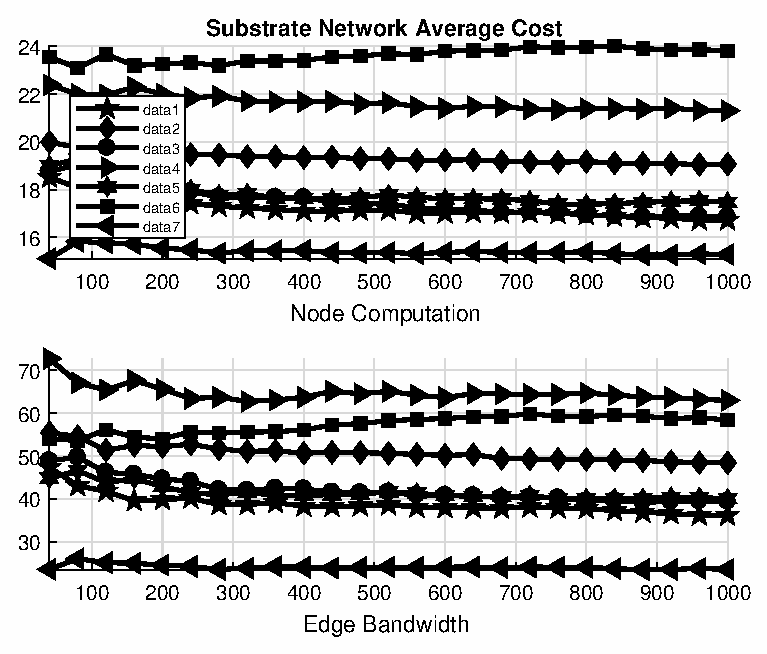
\includegraphics[width=\textwidth]{figures/CostAccumulateAverageSubstrateNetwork}
\caption{底层物理网络消耗资源的平均成本}\label{fig:CostAccumulateAverageSubstrateNetwork}
\end{minipage}
\begin{minipage}{0.4\textwidth}
\centering
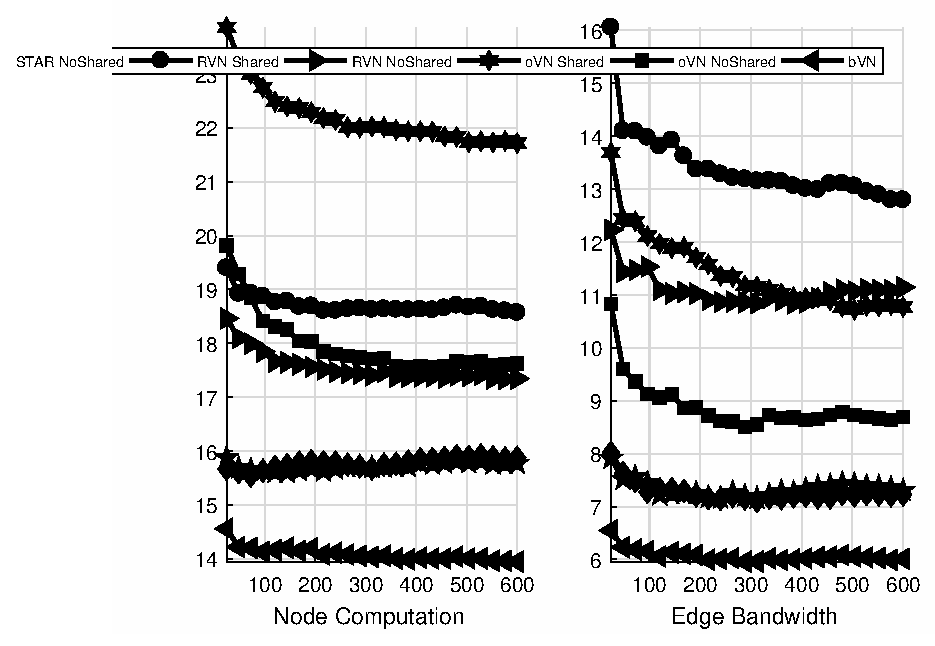
\includegraphics[width=\textwidth]{figures/RevenueAccumulateAverageVirtualNetwork}
\caption{虚拟网络获得需求的平均收益}\label{fig:RevenueAccumulateAverageVirtualNetwork}
\end{minipage}\vspace{\baselineskip}
\end{figure}
\end{frame}
